\documentclass[12pt]{article}

\newlength\tindent
\setlength{\tindent}{\parindent}
\setlength{\parindent}{0pt}
\renewcommand{\indent}{\hspace*{\tindent}}

%% packages
\usepackage{enumerate}
\usepackage{listings}
\usepackage{multicol}
\usepackage{amsmath}
\usepackage{caption}
\usepackage{subcaption}
\usepackage[a4paper,margin=2cm]{geometry}
% \usepackage[english, norsk]{babel}
\usepackage{fancyhdr}
\usepackage{pdfpages}
\usepackage{lastpage}
% \usepackage[demo]{graphicx}
\usepackage{graphicx}
\graphicspath{ {.} }


\date{}
\begin{document}

% intentionally empty
\author{Faculty of Mathematics and Natural Sciences}

\title{UNIVERSITY OF OSLO}

\maketitle 
\begin{center}
\textbf{Trial exam in GEO4300/9300 -- Geophysical Data Science}
\end{center}

This paper consists of \pageref{LastPage} pages including this page. \\


\pagebreak


%\pagebreak
\section{Random variables}

\begin{enumerate}[(a)] 
\item Explain or define the mean, median and mode of a random variable.
\item Explain or define a measure of dispersion of a random variable.
\item For bivariate random variables, explain how the Pearson correlation coefficient and the Spearman rank correlation coefficients are calculated and explain the differences between them. You may draw a simple sketch to illustrate the differences.
\end{enumerate}




\section{Hypothesis testing}
Based on two samples with respectively 1000 and 100 observations, the following estimates for mean and standard deviations have been obtained:

Sample 1 ($n_1=1000$): \hspace{0.3in} $\bar{x}_1=44.1$ \hspace{0.3in} $\sigma_1=11.3$

Sample 2 ($n_2=100$): \hspace{0.3in} $\bar{x}_2=48.0$ \hspace{0.3in} $\sigma_2=8.2$


\begin{enumerate}[(a)] 
    \item Test if the estimates for mean and standard deviation are significantly different. Use a significance level of 5\%.
	\item We make two types of errors in hypothesis testing. Explain these type I and type II errors, and illustrate graphically the relation between them.
\end{enumerate}



%\pagebreak
\section{Goodness-of-fit testing}
The table below shows July precipitation data ($P$ in inches) for $N=30$ years of observations between 1951 and 1980 in Ithaca, New York.

\begin{figure}[h!]
    \centering
    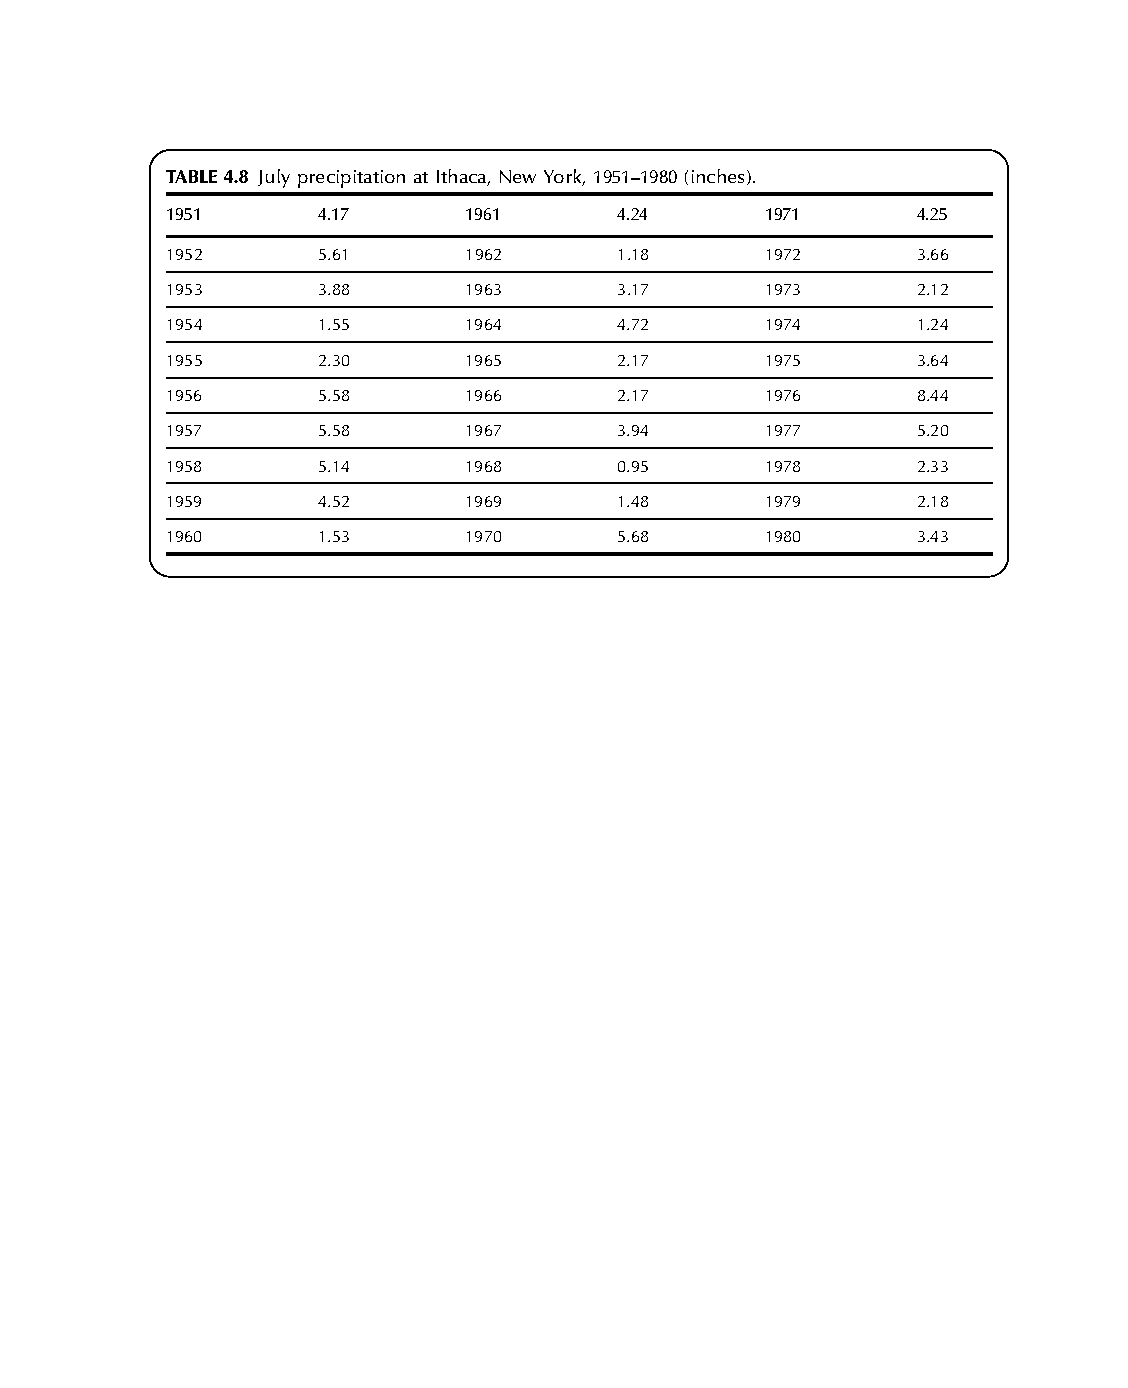
\includegraphics[width=.8\textwidth]{table48} 
%    \caption{}
\end{figure}

The mean value of the data is $\bar{P}=3.54$ inches and the standard deviation $s=1.77$ inches.

\begin{enumerate}[(a)] 
\item Bin the data in suitable classes and sketch the cumulative histogram of the dataset.
\item Use the Chi-square method to test the hypothesis that the data fit the normal distribution. Use a significance level of 5\%.
\end{enumerate}



\pagebreak
\section{Time series analysis}
Consider the following time series $X_t$ sampled at $n=70$ time steps:

\begin{figure}[h!]
    \centering
    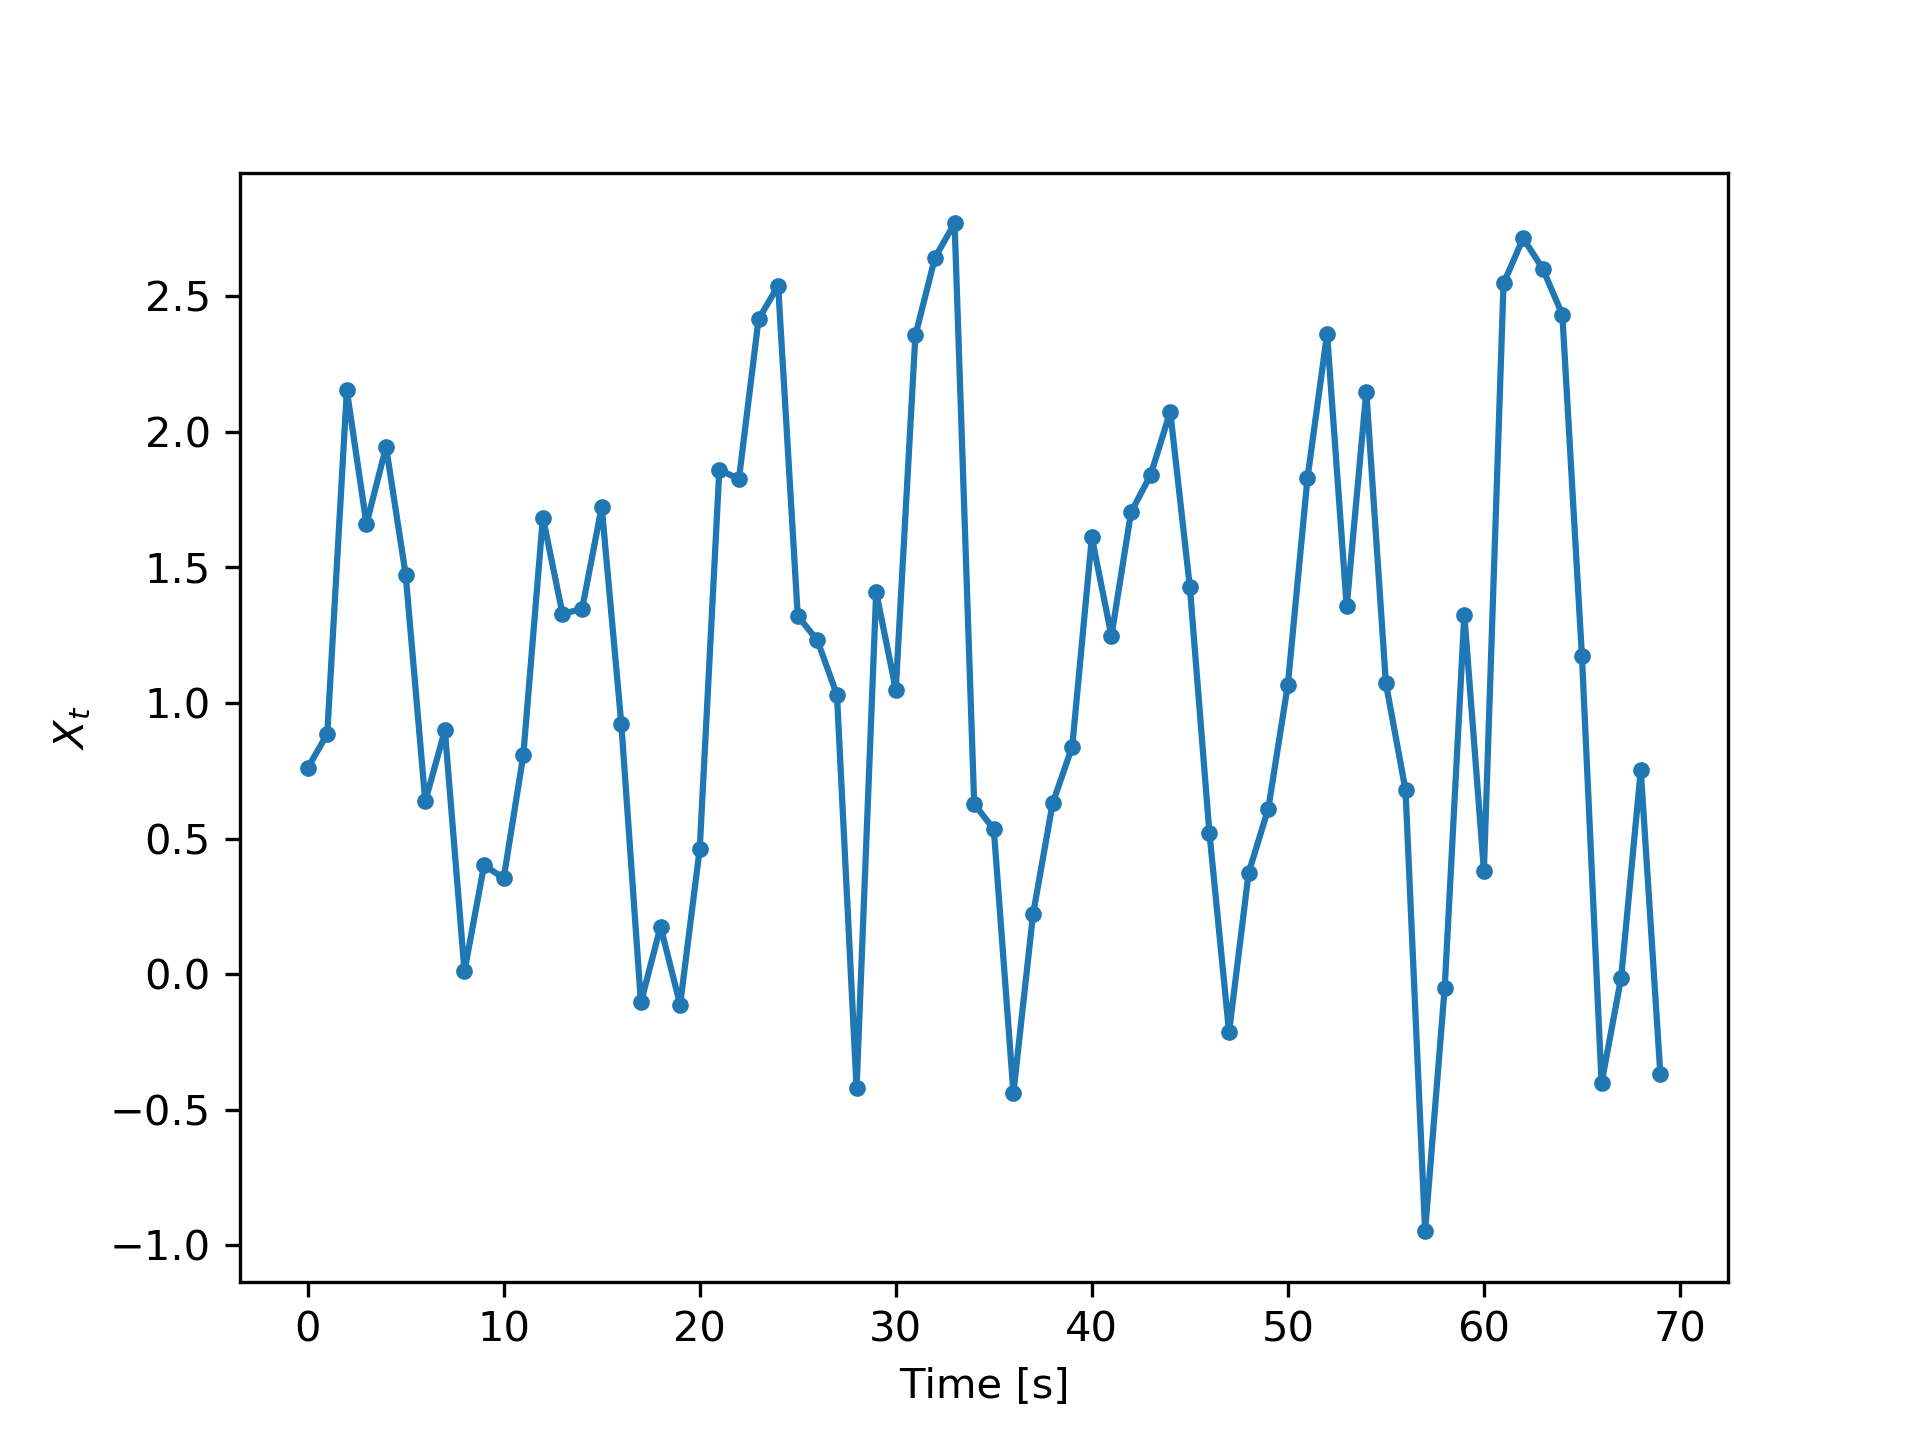
\includegraphics[width=.8\textwidth]{autocorrelation_y} 
%    \caption{}
\end{figure}


\begin{enumerate}[(a)]
\item The following three graphs show autocorrelation functions for lags $L \le 50$, defined as:
$$ r_L = \frac{1}{n-L} \sum_{t=1}^{n-L} (X_t-\bar{X}) (X_{t+L} - \bar{X}) / \frac{1}{n} \sum_{t=1}^n (X_t-\bar{X})^2$$

\begin{figure}[h!]
    \centering
    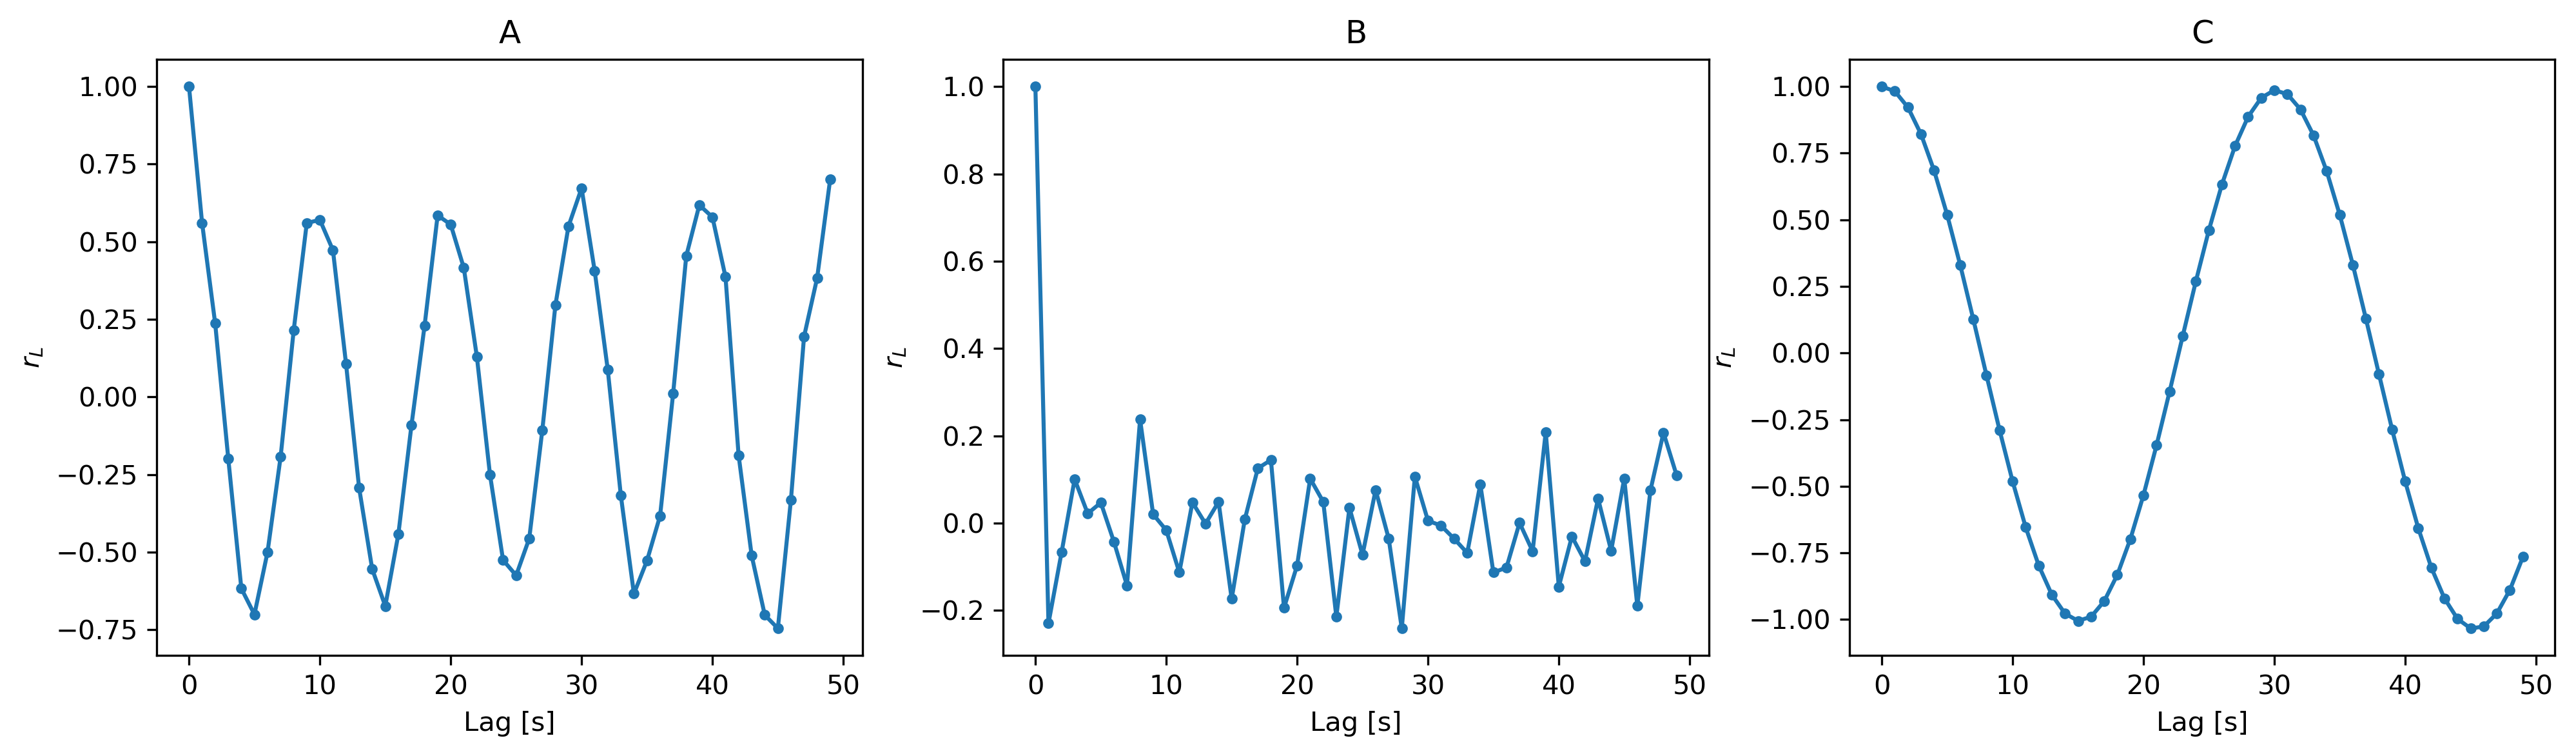
\includegraphics[width=.8\textwidth]{autocorrelation_rl} 
%    \caption{}
\end{figure}
Which one of them (A, B or C) shows the autocorrelation of $X_t$? Explain your answer.

\end{enumerate}



\pagebreak
\section{Machine learning}
\begin{enumerate}[(a)] 
\item What is the difference between supervised and unsupervised machine learning? Give an example of one model/learning algorithm and argue why you can categorize it as supervised (or unsupervised).
\item Explain the difference between the two main types of supervised machine learning: regression and classification. Give an example of each type.
\end{enumerate}



\end{document}











